%!TEX program = xelatex
\documentclass[11pt]{beamer}

\usepackage{amsfonts}
\usepackage{amsmath}
\usepackage{blindtext}
\usepackage{enumitem}
\usepackage{hyperref}
\usepackage{colortbl}
\usepackage{fancyvrb}
\usepackage{booktabs}
\usepackage{listings}

\newcommand{\ubar}[1]{\text{\underline{$#1$}}}

\hypersetup{pdfborder = {0 0 0}}

\usetheme{Green}

\title{Data Harvesting for Agriculture}
\author{CarpentryCon 2020 Lightning Talk}
\date{N E Davis · 2020-08-07}

\setcounter{showSlideNumbers}{1}

\newcommand{\correctstar}{\textcolor{CS101Midtone}{$\star$}}

\lstset{showstringspaces=false,language=python}

\newcounter{QuestionCounter}
\setcounter{QuestionCounter}{0}

\begin{document}
  \setcounter{showProgressBar}{0}
  \setcounter{showSlideNumbers}{0}

%%%%%%%%%%%%%%%%%%%%%%%%%%%%%%%%%%%%%%%%%%%%%%%%%%%%%%%%%%%%%%%%%%%%%%%%%%%%%%%%
%%%%%%%%%%%%%%%%%%%%%%%%%%%%%%%%%%%%%%%%%%%%%%%%%%%%%%%%%%%%%%%%%%%%%%%%%%%%%%%%
\frame{\titlepage}

%%%%%%%%%%%%%%%%%%%%%%%%%%%%%%%%%%%%%%%%%%%%%%%%%%%%%%%%%%%%%%%%%%%%%%%%%%%%%%%%
\begin{frame}[fragile]
\frametitle{Overview}

  “Our motivation for creating this workshop is the recent, rapid increase in the volume of data produced on farms and the use of such data for decision making by farmers.

  “After attending our workshop, you will be able to develop small computer programs of your own for analysis, visualization, and decision making, and will be able to share those programs with others.”
\end{frame}

%%%%%%%%%%%%%%%%%%%%%%%%%%%%%%%%%%%%%%%%%%%%%%%%%%%%%%%%%%%%%%%%%%%%%%%%%%%%%%%%
\begin{frame}[fragile]
\frametitle{Scope}
  \begin{enumerate}[label=\arabic*]
    \item  Non-academic audience
    \item  No prior programming assumed
    \item  Target:  Use or modify packaged scripts
  \end{enumerate}
\end{frame}

%%%%%%%%%%%%%%%%%%%%%%%%%%%%%%%%%%%%%%%%%%%%%%%%%%%%%%%%%%%%%%%%%%%%%%%%%%%%%%%%
\begin{frame}[fragile]
\frametitle{Topics}
  \begin{enumerate}[label=\arabic*]
    \item  R/R Studio basics
    \item  Geospatial data (QGIS)
    \item  Trial design
    \item  Weather history and soil types
  \end{enumerate}
\end{frame}

%%%%%%%%%%%%%%%%%%%%%%%%%%%%%%%%%%%%%%%%%%%%%%%%%%%%%%%%%%%%%%%%%%%%%%%%%%%%%%%%
\begin{frame}[fragile]
\frametitle{Products}
  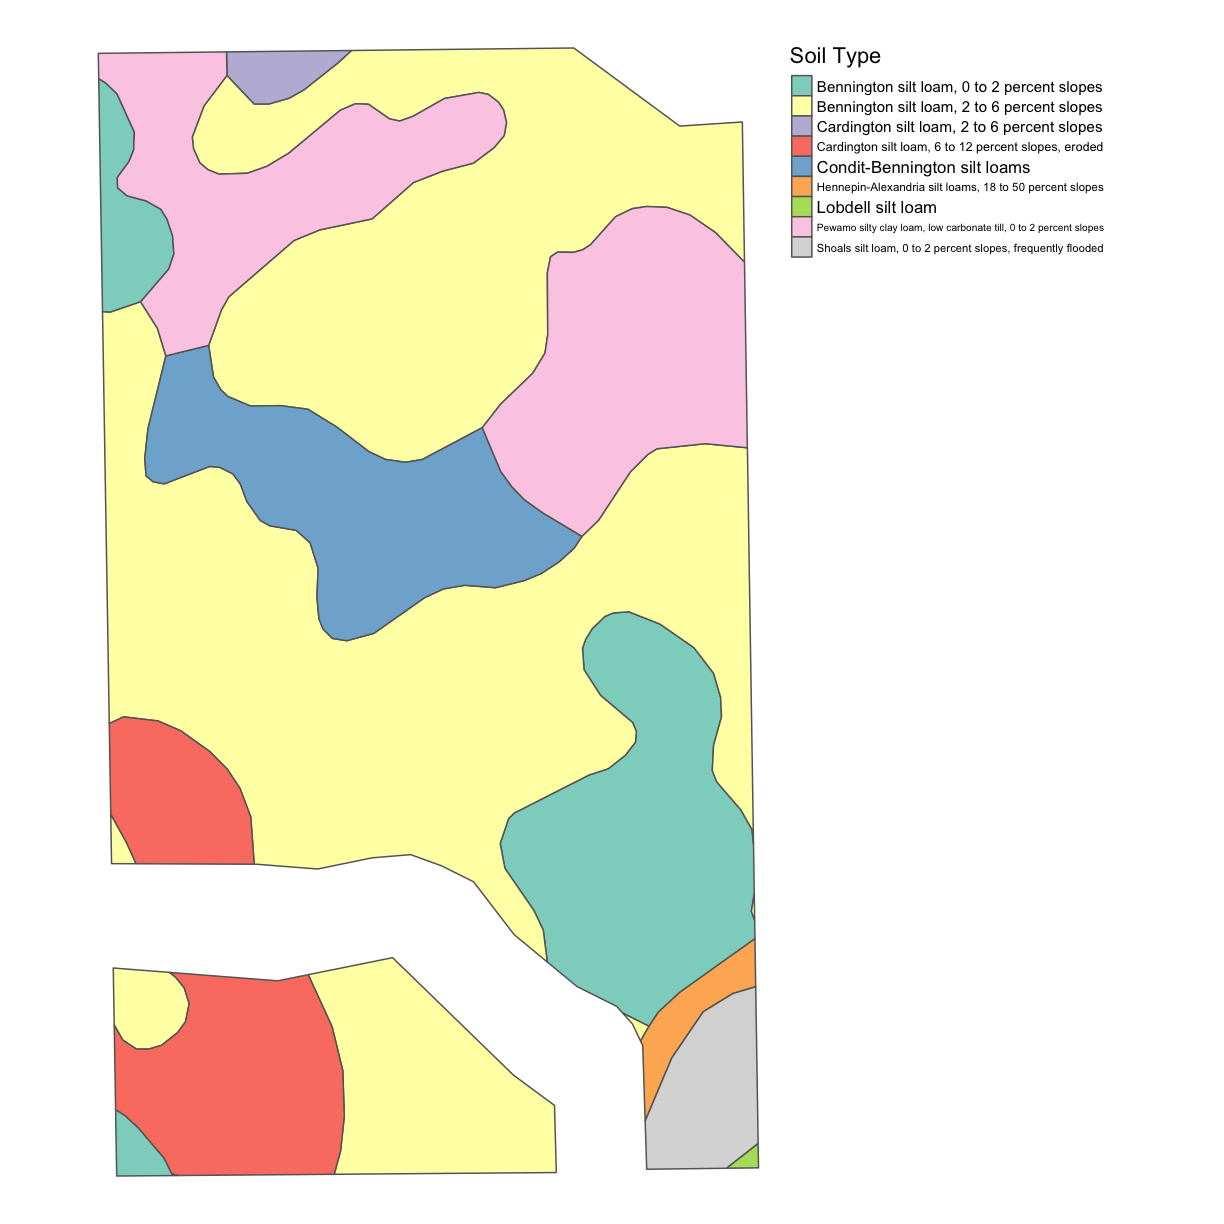
\includegraphics[height=0.75\textheight]{./img/rmd-map_soil_spatial-1}
\end{frame}

%%%%%%%%%%%%%%%%%%%%%%%%%%%%%%%%%%%%%%%%%%%%%%%%%%%%%%%%%%%%%%%%%%%%%%%%%%%%%%%%
\begin{frame}[fragile]
\frametitle{Products}
  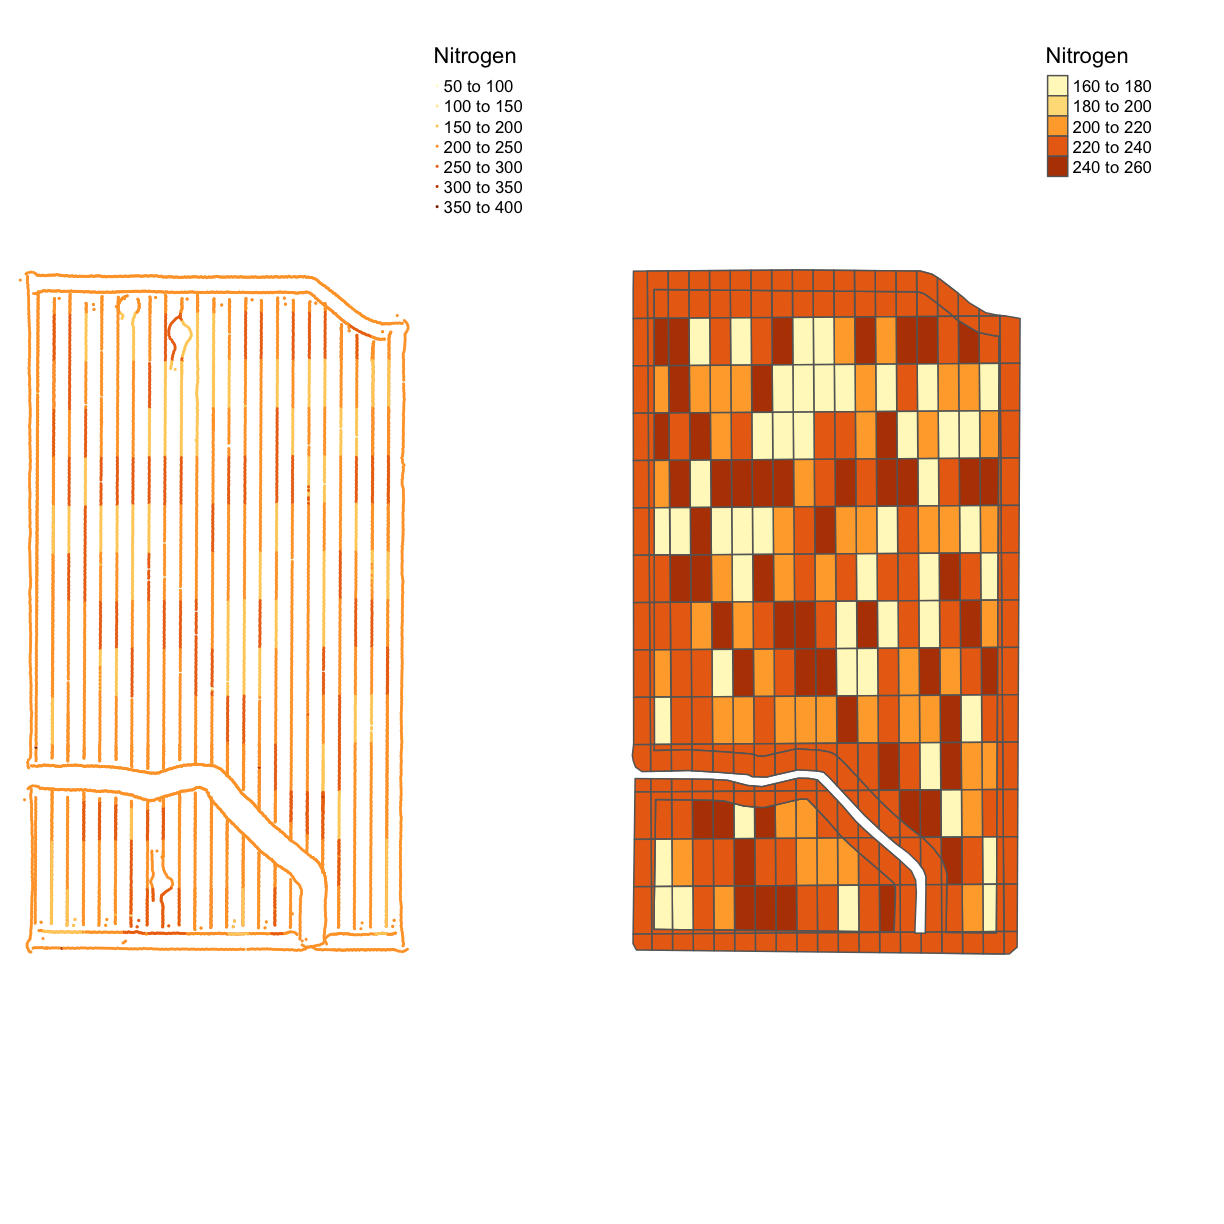
\includegraphics[height=0.75\textheight]{./img/rmd-nitrogenmap-2.png}
\end{frame}

%%%%%%%%%%%%%%%%%%%%%%%%%%%%%%%%%%%%%%%%%%%%%%%%%%%%%%%%%%%%%%%%%%%%%%%%%%%%%%%%
\begin{frame}[fragile]
\frametitle{Feedback}
  \begin{enumerate}[label=\arabic*]
    \item[+]  “Good intro to working with spatial data in R”
    \item[+]  “How using farm data can improve farming operations”
    \item[-]  Needs less emphasis on trials, more hands-on work with QGIS and mapping
    \item[-]  Needs more time working with own data
  \end{enumerate}
\end{frame}

%%%%%%%%%%%%%%%%%%%%%%%%%%%%%%%%%%%%%%%%%%%%%%%%%%%%%%%%%%%%%%%%%%%%%%%%%%%%%%%%
\begin{frame}[fragile]
\frametitle{Next Steps}
  \begin{enumerate}[label=\arabic*]
    \item  Refine focus for field operations
    \item  Include irrigation-based farming
    \item  Expand mapping operations and QGIS
    \item  Retool exercises for working with own data
  \end{enumerate}
\end{frame}

%%%%%%%%%%%%%%%%%%%%%%%%%%%%%%%%%%%%%%%%%%%%%%%%%%%%%%%%%%%%%%%%%%%%%%%%%%%%%%%%
\begin{frame}[fragile]
\frametitle{Finding Us}
  \begin{tabular}{c l}
    \begin{tabular}{c}
      
\includegraphics[width=36pt]{./img/github17.eps}
    \end{tabular}
    &
    \begin{tabular}{p{8cm}}
      {\Large data-carpentry-for-agriculture/ trial-lesson}
    \end{tabular}
  \end{tabular}
\end{frame}

\end{document}
